%!TEX root = ../../beamer.tex
\begin{frame}
\begin{columns}[c]
\begin{column}{0.5\textwidth}
\begin{block}{\textbf{Observe gene expression}}
\begin{small}
\begin{itemize}
\item disregarding the structure of their interactions, \textbf{genes} can be indexed as $L = \{1, \ldots, l \}$
\item taking into account interactions, a \textbf{gene regulatory network module} is a subset of genes $O \subseteq L$ and these can be collected into a covering of the genotype space $\mathcal{G}$ where $L = \cup_{O \in \mathcal{G}} O$
\item regardless of the level of observation the total number of \textbf{phenotype values} under consideration can be indexed as $P = \{ 1, \ldots, p \} $
%\item an observation of a gene can take on different forms at different levels of "phenotypic" evaluation
\end{itemize}
\end{small}
\end{block}
\end{column}
\begin{column}{0.5\textwidth}
\begin{center}
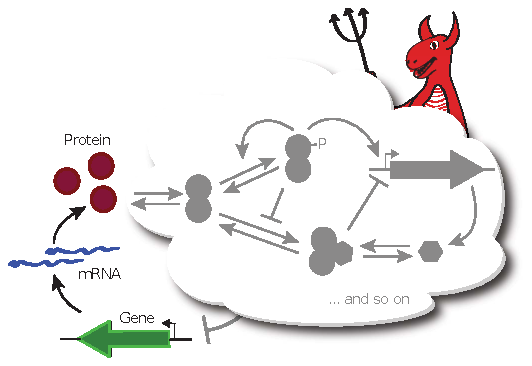
\includegraphics[width=0.8\textwidth]{fig/geneexpressiondemon.pdf}
\cite{Lestas2010}
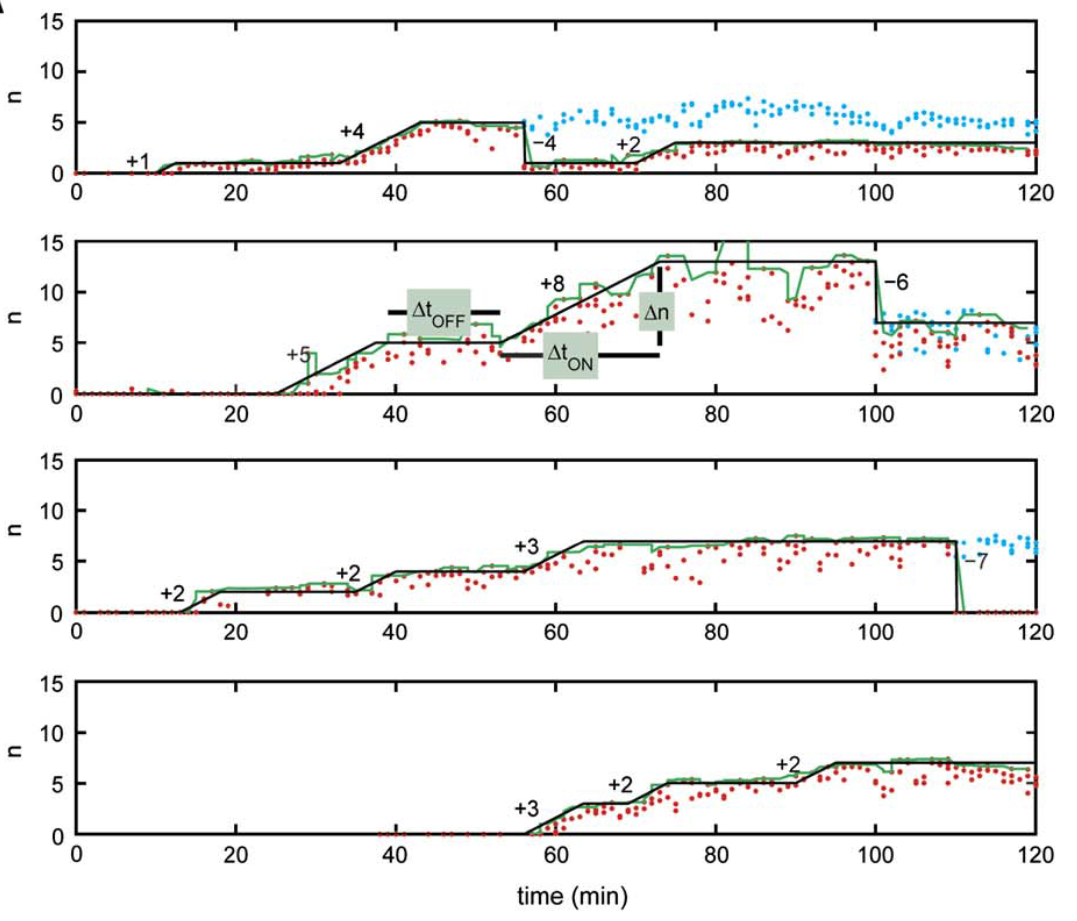
\includegraphics[width=0.8\textwidth]{fig/transcriptcounts.png}
\cite{Golding2005}
\end{center}
\end{column}
\end{columns}
\end{frame}
